\documentclass[11pt]{article}

\usepackage[utf8]{inputenc}
\usepackage{geometry}
\usepackage{color,graphicx,framed}
\usepackage{amsmath,amsfonts,amssymb}
\usepackage{listings}
\usepackage[section]{placeins}
\usepackage{pstricks,pst-tree,pst-node}
\usepackage{dsfont}
\usepackage{ulem}
\usepackage{nicefrac}

\title{Abschlussbericht\\Proseminar Algorithmen\\Vortrag :Parallele Sortierung}
\author{Patrick Winterstein,Björn Rathjen}
\date{SS14}

\begin{document}
\maketitle
\newpage
\tableofcontents
\newpage
\listoffigures
\listoftables
\section{Einführung}
Der Titel Paralleles Sortieren beschreibt zwei grundsätzliche Bestrebungen bei der Optimierung von Netzwerk- (hauptsächlich Routing)und Datenstruckturen (Listen, Wörterbücher, \dots). Somit ist die Motivation diesen Thema zu behandeln groß, da sie für die Projekt die Basis für dessen Geschwindigkeit legen kann. Für sich alleine sind diese von folgender Bedeutung :
\begin{description}
\item[Sortierung] Sortierung ist die Basis für jede Suche auf Daten und Ressourcen. Wenn diese nicht wenigstens einer groben Ordnung unterliegen können effiziente Algorithmen nicht angewendet werden, da keine Annahmen über den Zustand getroffen werden können.
\item[Parallelität] Durch den Aufwand von mehr Ressourcen kann ein Sortierprozess beschleunigt werden ohne die Korrektheit den Ergebnisses zu gefährden. Dabei ist Parallelität der Extremfall, der eine Maximierung des Datendurchsatzes erlaubt und somit in einer höheren Geschwindigkeit gegenüber sequentiellen Ansätzen resultiert.
\end{description}
\section{Grundlagen}

\subsection{Sortieren}
Als Grundlage um eine Menge M sortieren zu können muss eine Ordnungsrelation R vorhanden sein, diese schreibt eine Ordnung zwischen zwei Elementen vor. 
\begin{equation}
R \subseteq M \times M
\label{eq:Ordnung}
\end{equation}
Der Anspruch an diese Relation ist, dass diese Transitivität beinhaltet.
\begin{equation}
\forall x,y,z \in M : xRy \wedge yRz \Rightarrow xRz
\label{eq:transit}
\end{equation}
Würde eine dieser Voraussetzungen nicht erfüllt sein, so würde bei \eqref{eq:Ordnung} kein sortieren möglich sein, da keine Relation vorhanden ist, und bei \eqref{eq:transit} die Relation zweier Elemente untereinander keine Aussage über die Relation zu anderen Elementen aussagt. Daraus resultiert das das "sortierte" Ergebnis nur zu einem Element als sortiert betrachtet werden kann.
\subsection{Komparator}
Ein Komparator stellt den kleinsten Baustein dar, der eine zweielementige Menge entsprechend der auf ihr liegenden Ordnungsrelation sortiert ausgibt. Dieser ist wie folgt aufgebaut. Er besitzt zwei Eingangsleitungen auf dem die zu sortierenden Mengen eingegeben werden, den Vergleichen Teil der die Ordnungsrelation anwendet und die beiden Ausgangsleitungen auf den das sortierte Ergebnis ausgegeben wird. Beide werden in Abbildung \ref{fig:kompsoft} (Software, Seite \pageref{fig:kompsoft})) und Abbildung \ref{fig:komparator} (Hardware, Seite \pageref{fig:komparator}) dargestellt. Die Annahme für die folgenden Abbildungen ist dass das sortierte Ergebnis von oben nach unten größer wird.
\begin{figure}
\begin{center}
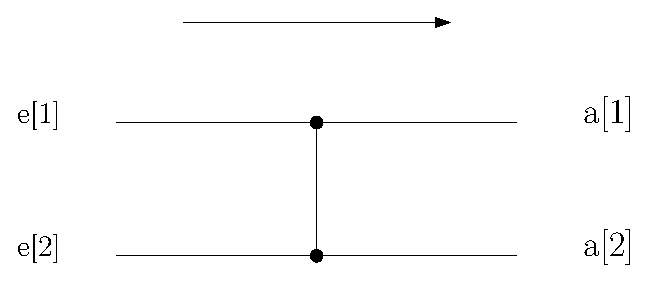
\includegraphics[scale=0.8]{Komparator1.eps}
\end{center}
\caption{Schema eines Komparators. e entspricht den Eingängen und a den Ausgängen. Der Pfeil gibt die Durchlaufrichtung an. Die waagerechten schwarzen Linien entsprechen den Datenleitungen, die senkrechte Linie zeigt die vergleichenden Teil an.}
\label{fig:komparator}
\end{figure}
\begin{figure}
\begin{lstlisting}[language=C,tabsize=4,numbers=left]
    void comp(chan in1, in2, out1, out2 Comparer{}){
        a := <- in1
        b := <- in2
        
        if (a < b){
            out1 <- a
            out2 <- b
            return void
        }
        out1 <- b
        out2 <- a
        return void
    }
\end{lstlisting}
\caption{Implementierung eines Komparators in Pseudocode (An Go angelehnt). inX entspricht den Eingangsleitungen, outX entspricht den Ausgangsleitungen, Comparer besagt, dass der Datentyp die beschriebenen Voraussetzungen (\eqref{eq:Ordnung} und \eqref{eq:transit}) erfüllt. "return void" zeigt, dass die Funktion nur die Ein- und Ausgänge verwendet.}
\label{fig:kompsoft}
\end{figure}
\FloatBarrier
\section{Sortiernetzwerk}
Die im vorherigen Abschnitt beschriebenen Voraussetzungen dienen nun als Grundlage dafür ein größeres Netzwerk aufzubauen das folgende Eigenschaften besitzt :
\begin{itemize}
\item mehrere Eingabeleitungen
\item mekrere Vergleicher
\item Ausgabe soll sortiert sein
\end{itemize}
Es wird noch kein Anspruch an Komplexität und Effizienz erhoben.
\FloatBarrier
\subsection{Aufbau}
Ein naiver Ansatz für den Aufbau des Netzwerks wird in Abbildung \ref{fig:kompnetsmall}(Seite \pageref{fig:kompnetsmall}) gezeigt. Die Anzahl der Leitungen wurde verdoppelt und die Anzahl der Komparatoren angepasst. In Abbildung \ref{fig:kompnetnumbex} (Seite \pageref{fig:kompnetnumbex}) wird der Vollständigkeit halber ein größeres Zahlenbeispiel gezeigt. Die Sortierung der vorher unsortierten Eingabe kann schrittweise verfolgt und überprüft werden.
\begin{figure}
\begin{center}
\begin{minipage}[l]{2cm}
Input
\end{minipage}
\begin{minipage}[c]{7cm}
\begin{center}
    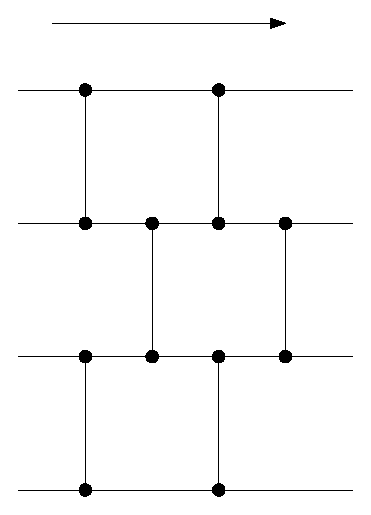
\includegraphics[scale=0.8]{bild2Komparatornetzwerk.eps}
\end{center}
\end{minipage}
\begin{minipage}[r]{2cm}
Output
\end{minipage}
\end{center}
\caption{Komparatornetzwerk mit mehreren Datenleitungen}
\label{fig:kompnetsmall}
\end{figure}
\begin{figure}
\begin{center}
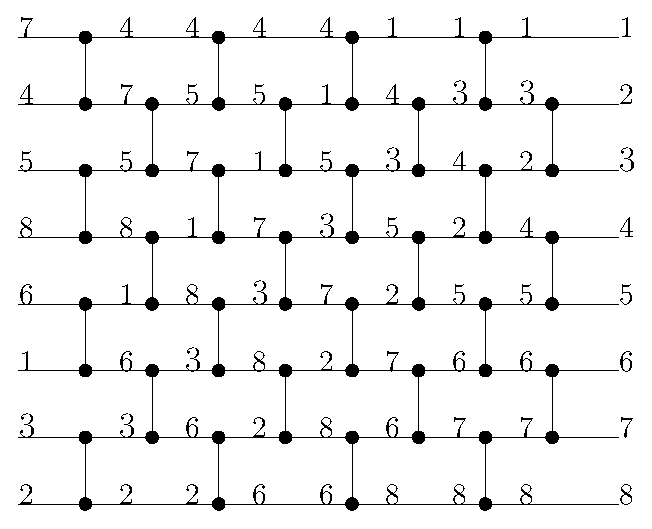
\includegraphics[scale=1]{bild2beispiel.eps}
\caption{Beispiel mit acht Datenleitungen dass einen schrittweisen Verlauf des sortierens zeigt und eine vollständig sortierte Ausgabe.}
\label{fig:kompnetnumbex}
\end{center}
\end{figure}
\FloatBarrier
\subsection{Korrektheit}
\subsubsection{Betrachtung der Analyse}
Problematisch bei der Überprüfung durch Beispiele ist die große Anzahl an der zu überprüfenden Fälle sehr groß ist. Im Beispiel in Abbildung \ref{fig:kompnetnumbex} (Seite \pageref{fig:kompnetnumbex}) bei einer Eingabemenge mit den Elementen 1 bis 8 wären dies 40320 unterschiedliche Fälle (diese Anzahl ist durch den Ausschluss, dass eine Zahl mehrfach vorkommt bereits reduziert worden) Allgemein ist die Anzahl $\nicefrac{n!}{(n-l)!}$, wobei n die möglichen Elemente und l die Anzahl der Datenleitungen ist. Nachfolgend wird nun eine einfachere Möglichkeit gezeigt, wie die Korrektheit überprüft werden kann.
\subsubsection{0,1-Prinzip}
Das 0,1-Prinzip ist ein Werkzeug zur Überprüfung, ob ein Sortiernetzwerk alle Eingaben richtig sortiert. Dabei werden die verschiedenen möglichen Eingaben durch 0,1-Folgen äquivalente (Zuweisung wird um Beweis gezeigt) und somit festgestellt, ob die simulierten Eingaben auch sortiert werden würden. 
\paragraph{Lemma}
Wenn es eine Folge A gibt, die ein Sor\-tier\-netz\-werk nicht sortiert, so existiert auch eine 0,1-Folge, die von diesem Netzwerk nicht sortiert wird.
\paragraph{Beweis} Geführt wird ein Beweis durch Widerspruch. 
\begin{enumerate}
\item[i)] Annahme : Wenn ein Sortiernetzwerk / Algorithmus eine Eingabe nicht sortiert, so sortiert er trotzdem alle 0,1-Folgen.
\item[ii)] Voraussetzungen : \begin{itemize}
\item Eingabefolge $E = e_0 \dots e_l$
\item sortiere Eingabefolge $ S = s_1 \dots s_l$
\item unsortierte Ausgabefolge von E $ U = u_1 \dots u_l $
\item kleinster Index an dem $u_k \neq s_k$ 
\end{itemize}
\item[iii)] Folgerungen aus ii) :
\begin{eqnarray}
u_i = s_i & & \forall 0 \neq i < k \\
u_r = s_k & & \text{mit } r > k
\end{eqnarray}
\item[iv)] Funktion die ein 0,1 Folge aus beliebiger anderer Folge erstellt. Die Konstante, die dazu verwendet wird ist in diesem Fall $s_k$.
\begin{equation}
f(e) = \begin{cases} 0 , & if \;\; e_i \leq s_k \\
    1 , & if \;\; e_i > s_k
    \end{cases}
\label{eq:cases}
\end{equation}
\item[v)] Wendet man die Funktion nun auf die Eingabe / Ausgabe an so entsteht eine 0,1-Folge der Form 
\begin{equation}
00 \dots 01_k\dots0_r \dots
\label{eq:01folge}
\end{equation}
\item[vi)] Folgerung : \\
$\Rightarrow$ die Folge ist unsortiert.\\
$\Rightarrow$ Widerspruch zur Annahme
\end{enumerate}
\paragraph{Vorteile} Durch das Anwenden des 0,1-Prinzips wird die Anzahl der Testfälle von 
\begin{equation}
n! \rightarrow 2^l
\label{eq:fallred}
\end{equation} 
reduziert. Daraus resultiert auch das mit größerer Sicherheit getestet werden kann und somit auch sauberer Testcode sauberer geschrieben werden kann.
\FloatBarrier
In einem Beispiel in Abbildung \ref{fig:01ex} (Seite \pageref{fig:01ex}) wird die Zuweisung mit $s_k = 6$ demonstriert und die anschließende Sortierung. 
\begin{figure}
\begin{center}
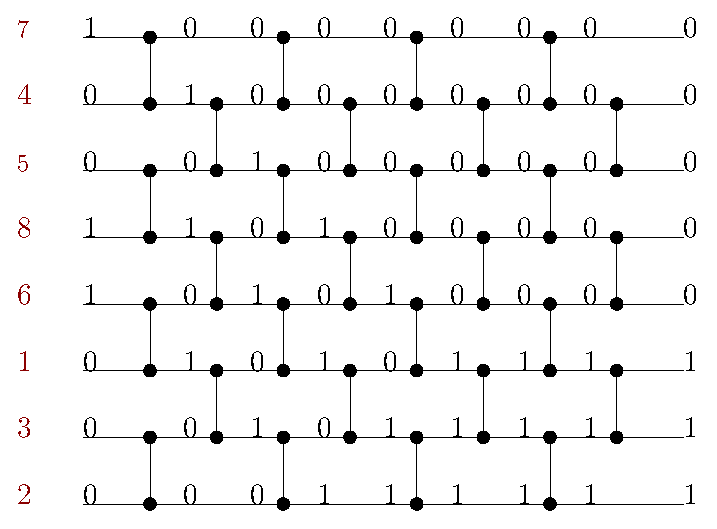
\includegraphics[scale=0.75]{01beispiel.eps}
\end{center}
\caption{Beispiel für das 0,1-Prinzip. Folge wird auf das Beispiel aus Abbildung \ref{fig:kompnetnumbex} (Seite \pageref{fig:kompnetnumbex}) angewendet. Es zeigt, dass das Resultat für die gewählte Konstante sortiert ist. Genauso zeigt es auch das bis Schritt 5 die Folge nicht sortiert ist.}
\label{fig:01ex}
\end{figure}
\subsection{Übertragung von Sortieralgorithmen auf ein Sortiernetzwerk}
\subsubsection{Bubblesort}
\FloatBarrier
Netzwerkimplementierung (\ref{fig:bubblesort} Seite \pageref{fig:bubblesort}) entspricht der Softwareimplementierung. Die Datenleitungen entsprechen den Indizes einer Liste von oben nach unten. Die Vergleiche folgen dem Algorithmus, Optimierungen in Form von Parallelen Vergleichen wurden bereits vollzogen.
\begin{figure}
\begin{center}
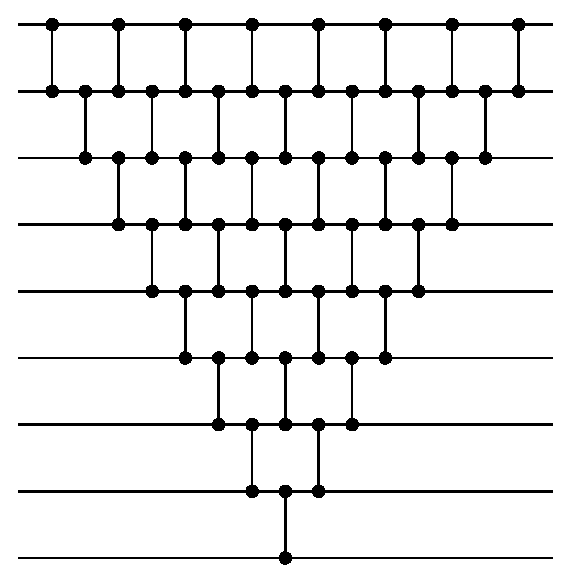
\includegraphics[scale=0.8]{bubblesort.eps}
\end{center}
\caption{Bubblesort: Bubblesort mit parallelen Vergleichen.}
\label{fig:bubblesort}
\end{figure}
\FloatBarrier
\subsubsection{Quicksort , Mergesort}
Bei der Implementierung schnellere Algorithmen zu implementieren entstehen durch direkte Umwandlung Probleme. 
\begin{description}
\item[Quicksort] Bei Quicksort wird vorweg ein Pivotelement gewählt nach dem die übrigen Werte auf zwei Listen aufgeteilt werden. Dies stellt in einem starren Netzwerk ein Problem dar, da die Größen dieser Listen von der Eingabe abhängen, und somit nach dem ersten Vergleich die Position den Pivot nicht mehr festgelegt ist. 
\item[Mergesort] Bei Mergesort wird die Eingabe in maximal 2-elementige Listen unterteilt, der danach dynamische merge-Prozess lässt sich nicht 1:1 auf ein starres Netzwerk übertragen
\end{description}
Dies wird in Abbildung \ref{fig:mergesort} (Seite \pageref{fig:mergesort}) verdeutlicht.
\begin{figure}
\begin{center}
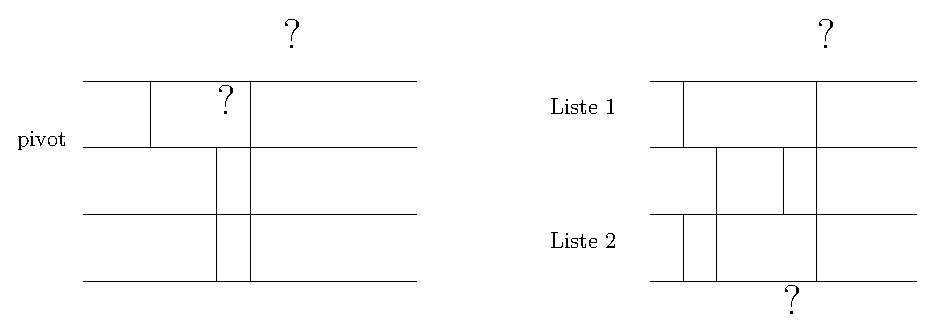
\includegraphics[scale=0.8]{mergesort.eps}
\end{center}
\caption{Auf der linken Seite ist der Versuch Quicksort, auf der rechten Seite Mergesort zu implementieren zu sehen}
\label{fig:mergesort}
\end{figure}
\subsection{Biton-Sortierer}
\subsection{Odd-Even-Mergesort}
\section{Laufzeit}
\subsection{Herleitung}
\section{Resultat}
\subsection{Vergleich zu Softwaresortierung}
\section{Anhang}
\subsection{Text-Quellen}
\subsection{Bild-Quellen}
\end{document}

\begin{figure}
\begin{center}
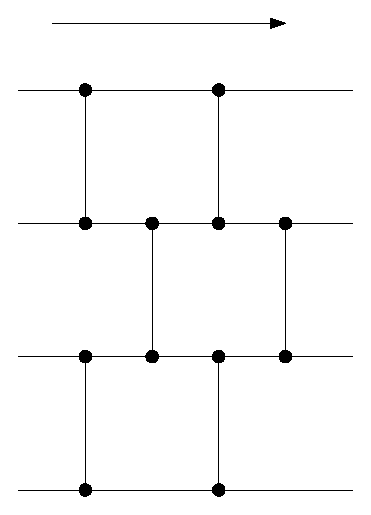
\includegraphics[scale=0.8]{bild2Komparatornetzwerk.eps}
\end{center}
\caption{ } %hier beschreibung
\label{fig:kompnetz2}
% für Referenz nächste Zeil kopieren
% Abbildung \ref{fig:kompnetz2} (Seite \pageref{fig:kompnetz2})
\end{figure}

\begin{figure}
\begin{center}
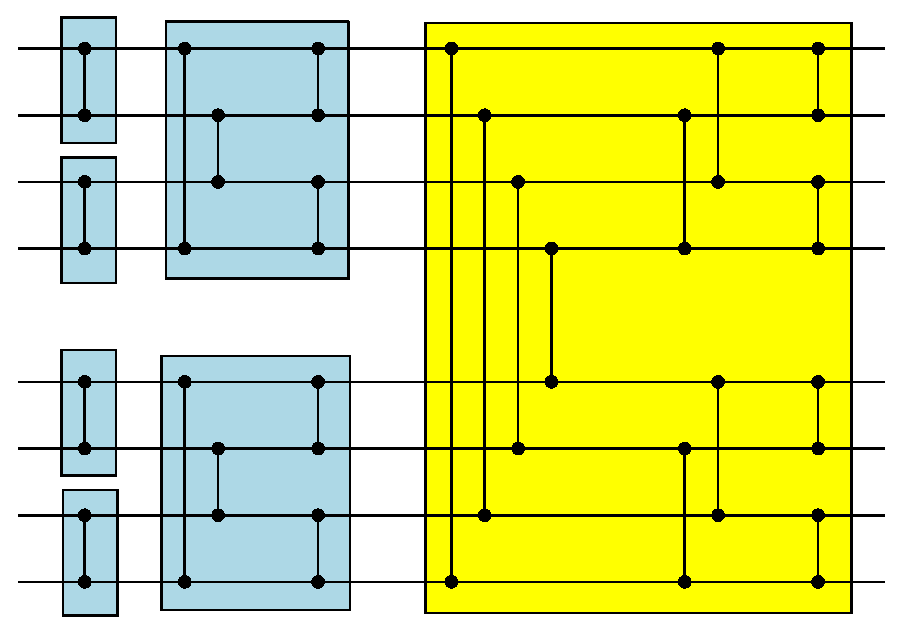
\includegraphics[scale=0.8]{biton1.eps}
\end{center}
\caption{ } %hier beschreibung
\label{fig:biton1}
% für Referenz nächste Zeil kopieren
% Abbildung \ref{fig:biton1} (Seite \pageref{fig:biton1})
\end{figure}

\begin{figure}
\begin{center}
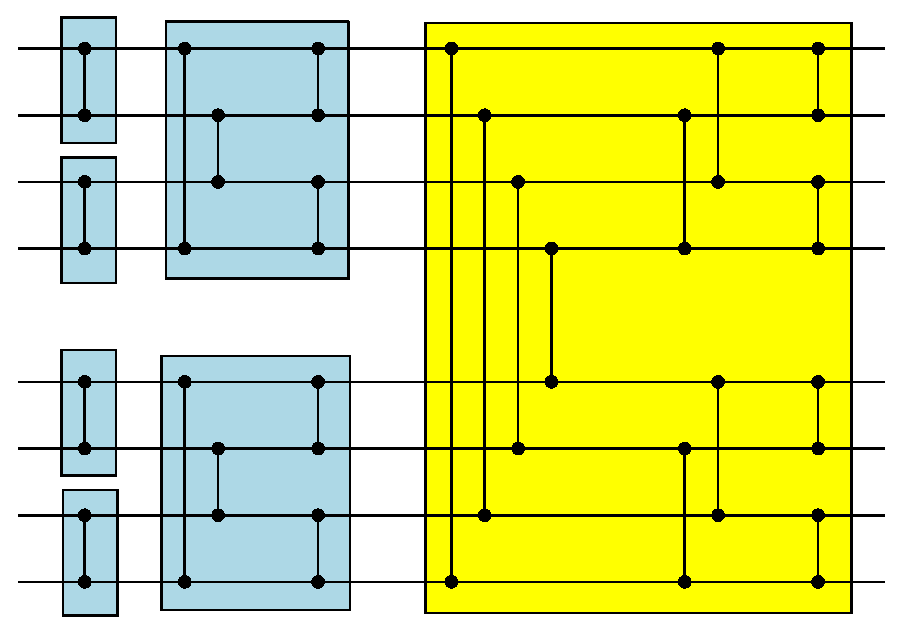
\includegraphics[scale=0.8]{biton2.eps}
\end{center}
\caption{ } %hier beschreibung
\label{fig:biton2}
% für Referenz nächste Zeil kopieren
% Abbildung \ref{fig:biton2 (Seite \pageref{fig:biton2)
\end{figure}

\begin{figure}
\begin{center}
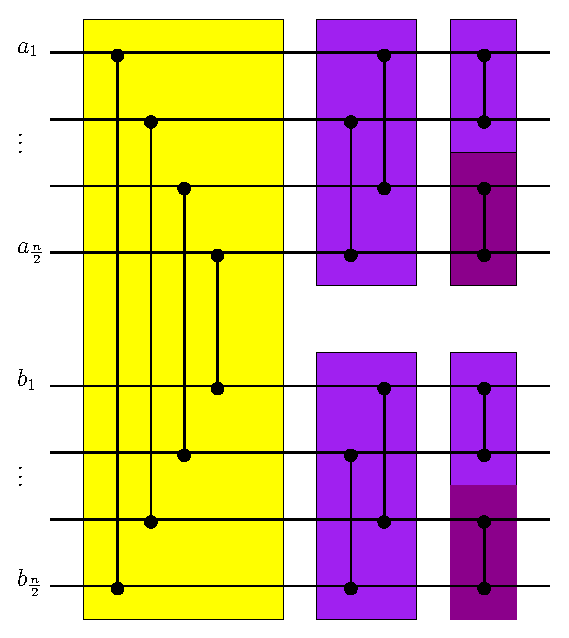
\includegraphics[scale=0.8]{bitonmischer.eps}
\end{center}
\caption{ } %hier beschreibung
\label{fig:bitonmischer}
% für Referenz nächste Zeil kopieren
% Abbildung \ref{fig:bitonmischer} (Seite \pageref{fig:bitonmischer})
\end{figure}